\documentclass[11pt, a4paper, twoside]{article}   	% use "amsart" instead of "article" for AMSLaTeX format

\usepackage{geometry}                		% See geometry.pdf to learn the layout options. There are lots.
\usepackage{pdfpages}
\usepackage{caption}
\usepackage{minted}
\usepackage[german]{babel}			% this end the next are needed for german umlaute
\usepackage[utf8]{inputenc}
\usepackage{color}
\usepackage{graphicx}
\usepackage{titlesec}
\usepackage{fancyhdr}
\usepackage{lastpage}
\usepackage{hyperref}
\usepackage[autostyle=false, style=english]{csquotes}
\usepackage{mathtools}
\usepackage{tabularx}
% http://www.artofproblemsolving.com/wiki/index.php/LaTeX:Symbols#Operators
% =============================================
% Layout & Colors
% =============================================
\geometry{
   a4paper,
   total={210mm,297mm},
   left=20mm,
   right=20mm,
   top=20mm,
   bottom=30mm
 }	

\definecolor{myred}{rgb}{0.8,0,0}
\definecolor{mygreen}{rgb}{0,0.6,0}
\definecolor{mygray}{rgb}{0.5,0.5,0.5}
\definecolor{mymauve}{rgb}{0.58,0,0.82}

\setcounter{secnumdepth}{4}


% the default java directory structure and the main packages
\newcommand{\xtextSrcDir}{../src/eclipse/at.ooe.fh.mdm.herzog.dsl.proj.ProjectGenerator/src/at/ooe/fh/mdm/herzog/dsl/proj/}
\newcommand{\uiSrcDir}{../src/eclipse/at.ooe.fh.mdm.herzog.dsl.proj.ProjectGenerator.ui/src/at/ooe/fh/mdm/herzog/dsl/proj/ui/}
\newcommand{\imageDir}{./images/}
% =============================================
% Code Settings
% =============================================
\newenvironment{code}{\captionsetup{type=listing}}{}
\newmintedfile[xSourceFile]{text}{
	linenos=true, 
	frame=single, 
	breaklines=true, 
	tabsize=2,
	numbersep=5pt,
	xleftmargin=10pt,
	baselinestretch=1,
	fontsize=\footnotesize
}
\newmintedfile[javaSourceFile]{java}{
	linenos=true, 
	frame=single, 
	breaklines=true, 
	tabsize=2,
	numbersep=5pt,
	xleftmargin=10pt,
	baselinestretch=1,
	fontsize=\footnotesize
}
% =============================================
% Page Style, Footers & Headers, Title
% =============================================
\title{Übung 1}
\author{Thomas Herzog}

\lhead{Übung 1}
\chead{}
\rhead{
\includegraphics[scale=0.10]{FHO_Logo_Students.jpg}}

\lfoot{S1610454013}
\cfoot{}
\rfoot{ \thepage / \pageref{LastPage} }
\renewcommand{\footrulewidth}{0.4pt}
% =============================================
% D O C U M E N T     C O N T E N T
% =============================================
% =============================================
% 2016.10.13: 1 
% 2016.10.14: 2
% =============================================

\pagestyle{fancy}
\begin{document}
\setlength{\headheight}{15mm}
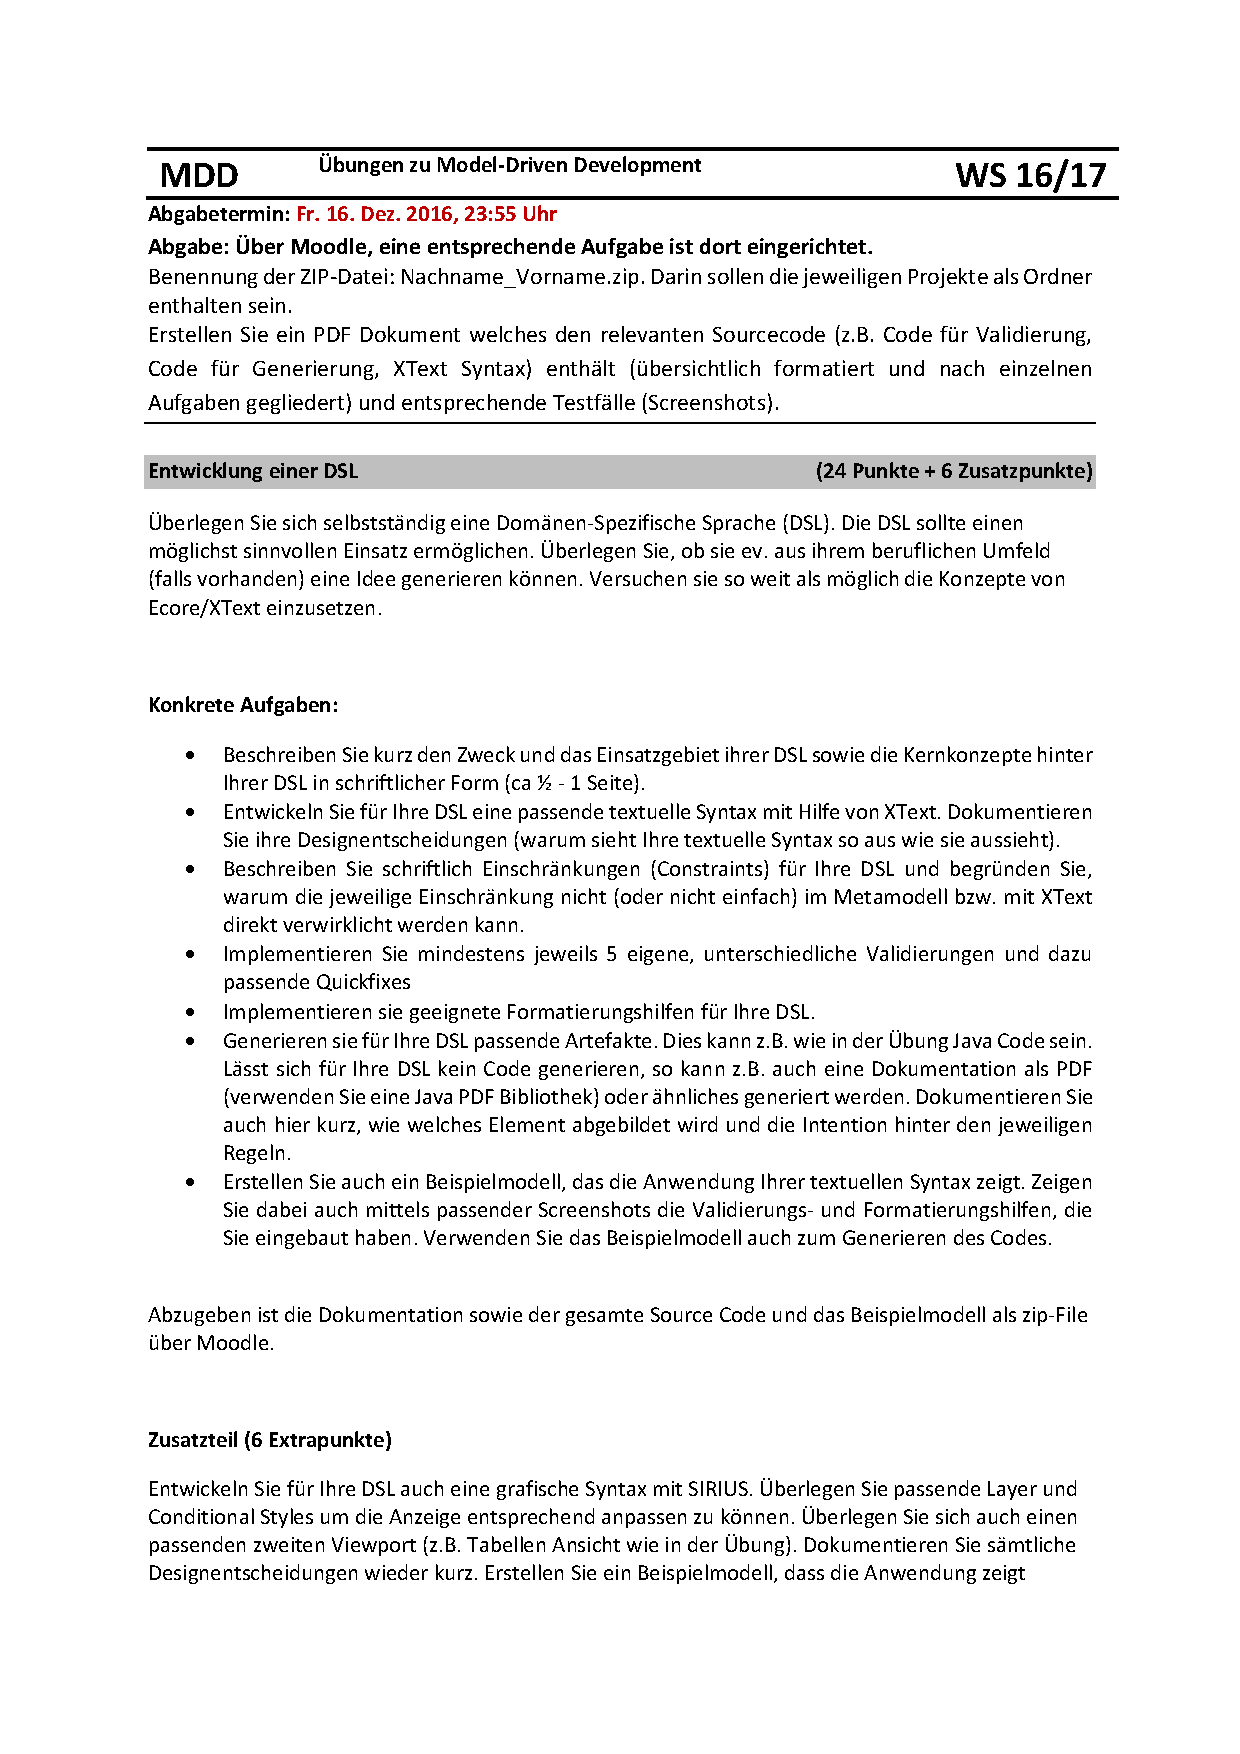
\includepdf[pages={1}]{Uebung.pdf}

\section{Beschreibung}
In dieser Übung wird eine \emph{DSL} entwickelt, mit der ein Modul für eine bestehende Anwendung beschrieben werden kann. Mit dieser Beschreibung wird eine Maven-Projektstruktur wie folgt aufgelistet erstellt:
\begin{itemize}
	\item\emph{\textbf{[MODULE\_KEY]}/model/pom.xml}
	\newline
	\emph{Parent} für alle Modell Projekte.
	
	\item\emph{\textbf{[MODULE\_KEY]}/model/jpa/pom.xml}
	\newline
	Das Projekt der \emph{JPA}-Modells.
	
	\item\emph{\textbf{[MODULE\_KEY]}/service/pom.xml}
	\newline
	\emph{Parent} für alle Service Projekte.
	
	\item\emph{\textbf{[MODULE\_KEY]}/service/api/pom.xml}
	\newline
	Das Projekt mit der Service Spezifikation

	\item\emph{\textbf{[MODULE\_KEY]}/service/impl/pom.xml}
	\newline
	Das Projekt mit der Service Implementierung.
\end{itemize}
\ \newline
Es können folgende \emph{Java}-Ressourcen definiert werden:
\begin{itemize}
	\item\textbf{\emph{MessageBundles}} sind Beschreibungen von Klassen, die sprachspezifische Texte für einen Schlüssel und eine \emph{Locale} verwalten.
	
	\item\textbf{\emph{Observers}} sind Beschreibungen von Beobachtermethoden, die mittels einen \emph{Delegate} auf einem definierten \emph{CDI}-Event reagieren können.
	
	\item\textbf{\emph{JpaConfig}} ist die Beschreibung des \emph{JPA}-Projekts, dem \emph{Observer} und \emph{MessageBundles} hinzugefügt werden können.
	
	\item\textbf{\emph{ServiceConfig}} ist die Beschreibung der \emph{Service}-Projekte, dem \emph{Observer} und \emph{MessageBundles} hinzugefügt werden können.
\end{itemize}
\ \newline
Das Ziel dieser \emph{DSL} ist es den initialen Aufwand beim erstellen eines Moduls für eine bestehende Anwendung zu erleichtern. Ein Module besteht aus mehreren \emph{Maven}-Projekten, die Mühsam erstellt werden müssen. Mit dieser \emph{DSL} kann ein Modul einfach beschrieben werden und daraus einen \emph{Maven}-Projektstruktur zu erstellen.


\section{XTEXT Grammatik}
\begin{code}
	\caption{ProjectGeneratorDsl.xtext}
	\xSourceFile{\xtextSrcDir/ProjectGeneratorDsl.xtext}
	\label{src:xtext-grammar}
\end{code}
\ \newline

\subsection{Regeln}
Die gesamte Konfiguration befindet sich im Wurzelobjekt des Typ Modul, das ein Modul beschreibt. Objekte, die in mehreren Objekten referenziert werden können, werden auf Ebene des Moduls einmalig beschrieben und dann von anderen Objekten referenziert \emph{(Observer, Localized)}. Sofern ein Name benötigt wird, wurde das Attribut Name den Regeln, die Objekte beschreiben, hinzugefügt, wobei der Name ebenfalls als Schlüssel für diese Objekte fungiert, damit diese Objekte referenziert werden können. Die einzelnen Regeln bilden Objekte, dessen \emph{Java}-Klassenbibliotheken bei der Validierung, Quickfixes und Generatoren verwendet werden.
 
\subsection{Konstanten}
Die Konstanten, wie die unterstützten \emph{Locale}, boolsche Zustände und \emph{Observer} spezifische Konstanten wurden als Aufzählungen abgebildet. Es wurde darauf geachtet, das über die Zeichenkettenrepräsentation der Aufzählungen sich leicht die \emph{Java}-Datentypen erstellen lassen.

\subsection{Terminal Regeln}
Die Terminal Regeln wurden eingeführt, damit die Klassennamen für die \emph{Observer}-Beschreibungen einen gültigen voll qualifizierten  \emph{Java}-Klassennamen darstellen und damit die Schlüssel der sprachspezifischen Einträge einer \emph{Localized}-Beschreibung, der Konvention von Schlüsseln einer \emph{Properties}-Datei folgen.
\newpage
\section{Constraint}
Folgende Auflistung beschreibt die implementierten Validierungen:
\begin{itemize}
	\item\textbf{\emph{Leere Beschreibung}}: Es wurde eine Validierung eingeführt, die auf eine leere Beschreibung eines Moduls prüft, damit ein \emph{Quickfix} eine initiale Beschreibung erstellen kann.
	
	\item\textbf{\emph{Duplikate Namen}}: Da die Namen vom Datentyp \emph{ID} sind, wurde zusätzlich eine Prüfung eingeführt, ob die Namen bereits vergeben wurden. \emph{(Observer, Localized)}
	
	\item\textbf{\emph{Camel case Namen}}: Da die Namen vom Datentyp \emph{ID} sind, wurde zusätzlich eine Prüfung eingeführt, ob die Namen in \emph{camel case} sind.
	
	\item\textbf{\emph{Duplikate LocaleEntry Einträge}}: Es wurde eine Validierung eingeführt, die prüft ob es Duplikate sprachspezifischen Einträge mit demselben Schlüssel gibt.
	
	\item\textbf{\emph{Doppelte Verwendung von \emph{Locale}}}: Es wurde eine Validierung eingeführt, die prüft ob eine \emph{Locale} innerhalb eines \emph{Bundles} definiert wurde.
	
	\item\textbf{\emph{Duplikate Referenzen}}: Es wurde eine Validierung eingeführt, die prüft ob es Duplikate bei den gesetzten Referenzen gibt.
	
	\item\textbf{\emph{Ungenutzte Objekte}}: Es wurde eine Validierung eingeführt, die prüft Objekte wie \emph{Observer} oder \emph{Localized} zwar definiert wurden aber nirgends referenziert werden.
	
	\item\textbf{\emph{Doppelte Objekt Ids}}: Es wurde eine Validierung eingeführt, die prüft ob Objekt Ids doppelt vergeben wurden \emph{(Observer, Localized)} Namen.
\end{itemize}
\ \newline
Mit einer Grammatik kann nicht beschrieben werden, dass es keine Duplikate bei den verwendeten Namen von Objekten in einer Auflistung gibt. Das ist so, da es sich hierum Semantik handelt und nicht Grammatik, ob ein Name nur einmalig oder mehrmalig vergeben werden darf.
\newline
\newline
Wenn das Attribut Name bereits als \emph{ID} festgesetzt wurde, dann kann nicht zusätzlich eine Terminalregel angewendet werden, die sicherstellt, das der Name auch z.B.: in \emph{camel case} ist. 
\newline
\newline
Wenn eine Auflistung definiert wurde wie \emph{(localizedEnums+=[Localized]+)}, dann kann mit der Grammatik nicht verhindert werden, das Duplikate bei den Referenzen angeben werden, da es sich hier auch um Semantik handelt. Das Attribut \emph{localizedEnums} wird als Liste abgebildet.
\newline
\newline
Das ein \emph{Localized} für eine \emph{Locale} nur einmal einen Eintrag definieren kann, ist eine Semantik, die auch nicht über die Grammatik abgebildet werden kann.
\section{Validation und Quickfix}
\begin{code}
	\caption{ProjectGeneratorValidator.xtend}
	\javaSourceFile{\xtextSrcDir/validation/ProjectGeneratorValidator.xtend}
	\label{src:xtend-validation}
\end{code}
\ \newpage

\begin{code}
	\caption{ProjectGeneratorQuickfixProvider.xtend}
	\javaSourceFile{\uiSrcDir/quickfix/ProjectGeneratorQuickfixProvider.xtend}
	\label{src:xtend-quickfix}
\end{code}
\section{Formatter}
\begin{code}
	\caption{ProjectGeneratorFormatter.xtend}
	\javaSourceFile{\xtextSrcDir/formatting2/ProjectGeneratorFormatter.xtend}
	\label{src:xtend-validation}
\end{code}
\ \newline

\end{document}
